\documentclass[a4paper, 11 pt]{article}
\usepackage[utf8]{inputenc}
\usepackage[T1]{fontenc}
\usepackage[slovene]{babel}
\usepackage{lmodern}
\usepackage{graphicx}
\usepackage{subcaption}



\title{Nanotorusi}
\author{Tomas Rode \\ Enej Kovač}

\begin{document}
\maketitle

\section{Navodila}

Nanotorus je 3-regularen graf na torusu. Vsak nanotorus lahko dobimo tako, da na šeskotni mreži enačimo nasprotni stranici danega paralelograma. Torej je vsak nanotorus določen z dvema vektorjema v ravnini, $(k,l)$ in $(m, n)$, za katera velja $k^2 + l^2 \neq 0$ in $m^2 + n^2 \neq 0$. Projekt je sestavljen iz štirih podnalog:

\begin{enumerate}
  \item V prvem delu naloge ustvarite funkcijo, ki v \textit{Sage} konstruira nanotorus, za dane $k, l, m$ in $n$.
  \item S pomočjo funkcij v \textit{Sage} preučite nekaj lastnosti nanotorusov: za dan $(k, l, m, n)$ določite število vozlišč, premer, tranzitivnost, ...
  \item Za $v \in V(T)$, poljubno vozlišče nanotorusa, določite število vozlišč na razdaljah $i:\ 1 \leq i \leq \textrm{diam}(T)$. Poiščite formulo za dane $i, k, l, m, n$.
  \item Naj bo $T$ nanotorus tipa $(k, l, m, n)$. Ugotovite ali obstaja nanotorus tipa $(k', 0, m', n')$, izomorfen $T$. Če obstaja, ugotovite odnos med $(k, l, m, n)$ in $(k', m', n')$.
\end{enumerate}

\section{Opravljeno delo (do 5. 11. 2019)}

S pomočjo objektnega programiranja sva v \textit{Sage} zapisala funkcijo, ki konstruira nanotorus s $k, l, m$ in $n$. Na sponjih slikah lahko vidimo nekaj primerov.

\begin{center}
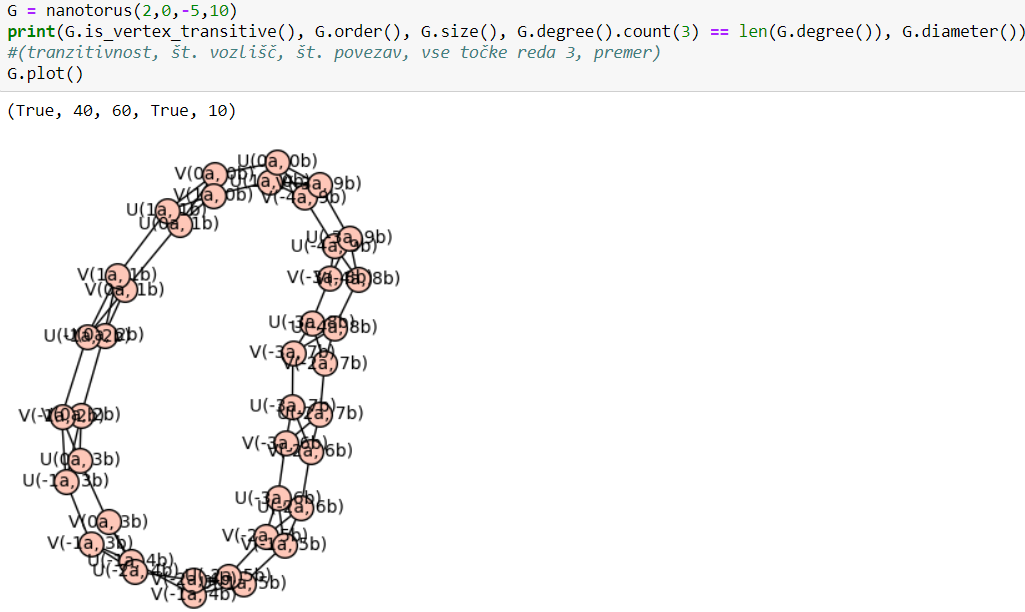
\includegraphics[width=10cm]{nano2}
\end{center}
\vspace{1cm}

Na prvi sliki sva dovolila, da \textit{Sage} prerazporedi točke po prosotru tako, da se čim bolje vidi oblika grafa. Pri tem se nekoliko izgubi šestkotna mreža, na kateri smo graf ustvarili. Pri vsakem grafu sva preverila še tranzitivnost, število vozlišč in povezav, red vozlišč in premer grafa.
\vspace{1cm}

\begin{center}
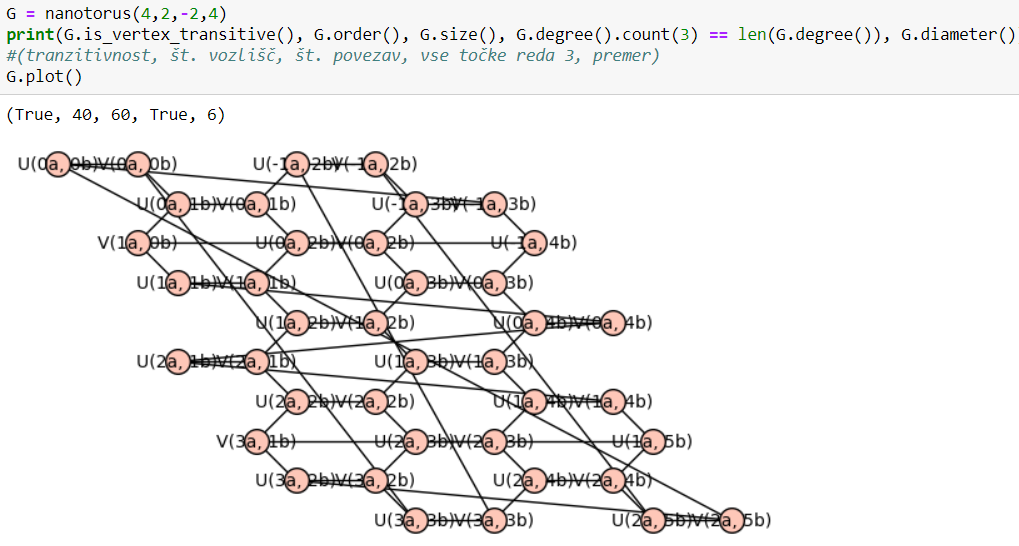
\includegraphics[width=10cm]{nano3}
\end{center}
\vspace{1cm}

Pri drugem grafu sva ohranila koordinate vozlišč na šestkotni mreži. Izmed vseh grafov je torej tukaj izvorna šestkotna mreža najbolj razvidna.
\vspace{1cm}

\begin{center}
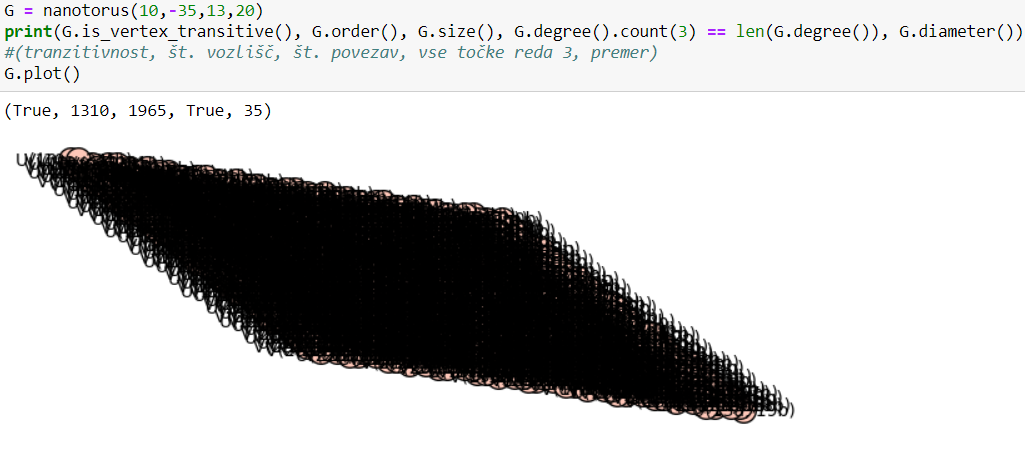
\includegraphics[width=10cm]{nano1}
\end{center}
\vspace{1cm}
\begin{center}
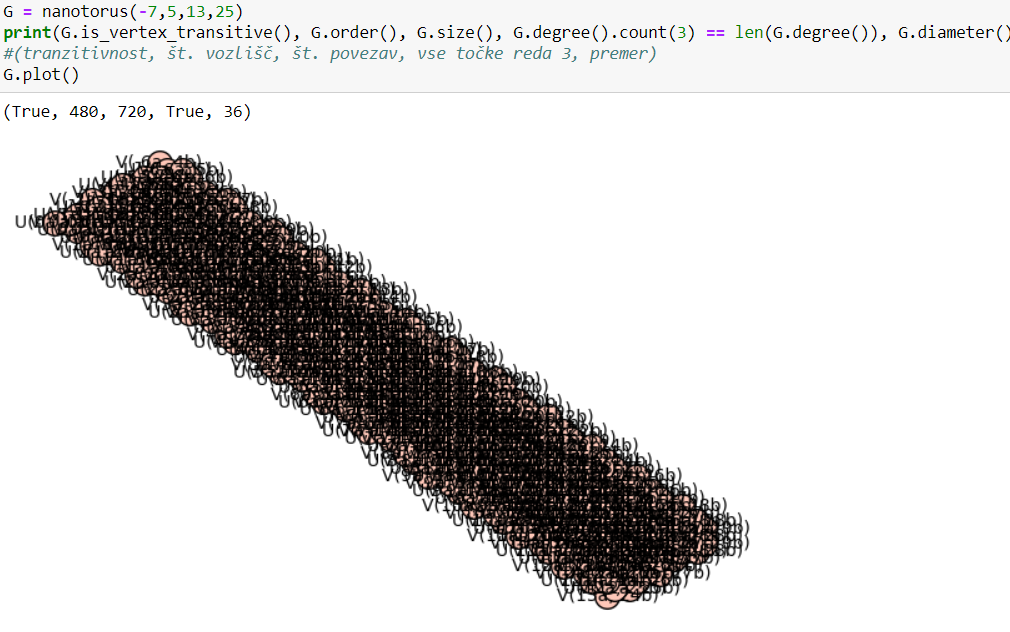
\includegraphics[width=10cm]{nano4}
\end{center}
\vspace{1cm}

Tretji in četrti graf imata veliko vozlišč, kar ju naredi zelo nepregledna, omogoči pa, da preverimo omenjene lastnosti nanotorusov tudi za velike grafe.






\section{Načrt za nadaljnje delo}

Delo bova nadaljevala pri nasledjih točkah iz navodil, torej bova najprej ugotavljala lastnosti nanotorusov. Iz teh ugotovitev bova potem preverjala, kakšne so razdalje v nanotorusu in kdaj sta nanotorusa izomorfna.


\end{document}
